\section{Motivation} \label{sec:motivation}

%%%
%
% Outline:
% - Current standard: terrestrial networking technology
%	- [Add papers on wired networking technology - glass fiber]
%	- Standard communication infrastructure works via cable.
%	- problem: expensive infrastructure, country borders, prone to risk [Paper] --> easy to attack wiring
%	- idea: solve most of these problems by putting up satellites which take over communication
%	- depending on height of satellite, it covers a big part of the earth's population
%	- with an antenna only, one could receive and transmit messages easily
% - Good idea, and governments already put up their networked satellite systems in order to have a fallback
%   in case some disaster appears.
%	- but not intended for the broad population
%	- intended for emergencies where little people use the system
% - in recent times, also businesses tried to use this idea and put their system up in the space, e.g,. HughesNet, ViaSat and Starlink
%	- but little is known, how well that actually works
%	- it was found that the height of satellites is the first influence
%		- GEO Satellites: Satellites at very high altitude
%		- LEO Satellites: Satellites at very low altitude
%	- Usually, GEO Satellites have a very high latency and cannot compete with LEO systems
%		- [Papers with Numbers for GEO and LEO]
%		- [Add papers that measure Starlink]
%	- However, little research is available to state clearly the performance and resilience of networked satellite systems
%		- therefore, the thesis proposed here wants to determine the current state of several networked satellite systems
%		- puts special remark on Starlink, as RIPE has many probes available for that in their measurement network
%
%%%

The internet plays a major role in our everyday's life. There are many technologies available that allow to connect to the web addressing different use cases (e.g., Wi-Fi for local area networks \cite{Henry2002} or \ac{FTTH} for high-speed wired connections to an end user's home \cite{Aleksic2010}).
However, there are several problems with such a setup. First, it requires wired infrastructure, which is quite expensive for networks in the wider area. For single end users, that is not affordable. Second, should the wired infrastructure be in place, it is vulnerable to attacks or natural catastrophes that render the service unusable.

Another emerging technology uses satellites as data transmission node. It is very resilient to human attacks or natural catastrophes as satellites are largely inaccessible. Therefore, governments installed dedicated satellite constellations to maintain communication in any given scenario. A satellite constellation is a group of artificial satellites that serve a specific purpose. Prominent examples of governmental satellite constellations are \textit{Beidou} and \textit{Galileo}.

Aside from crisis intervention, also businesses discovered opportunities. Providing communication over satellite allows users mobile access to information that usually require complex infrastructure. Users can access services like geographical data, radio frequencies, and even web access. Especially the demand for web access is growing, while companies failed at providing acceptable latencies in the past.

\begin{figure}
	\label{fig:satellitegrowth}
	\centering
	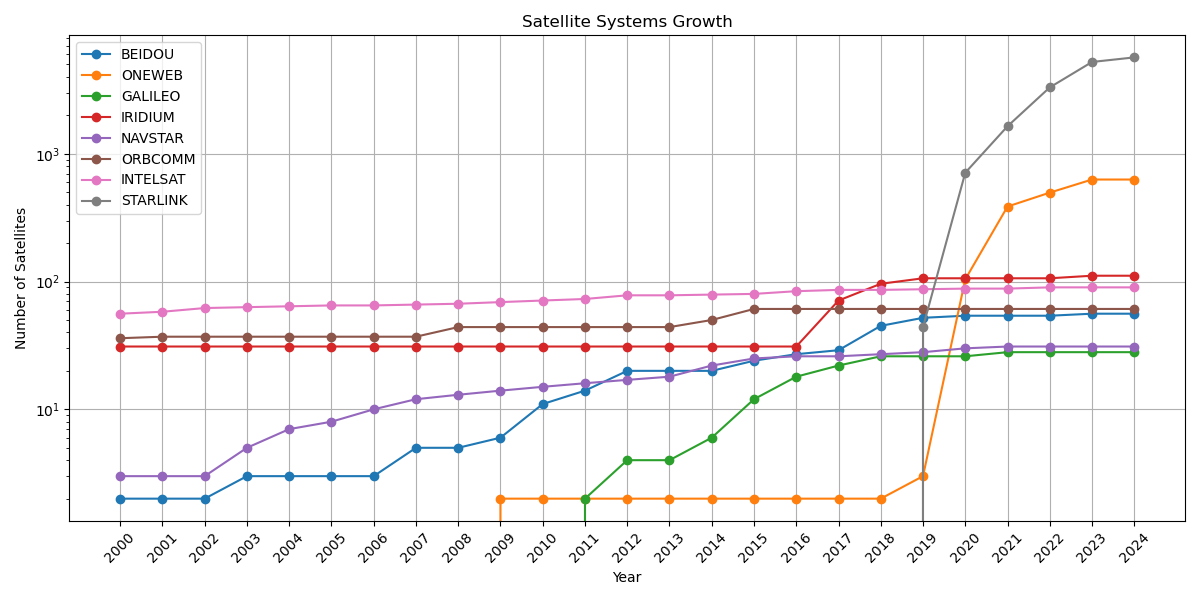
\includegraphics[width=\textwidth]{./chapters/img/satellite-growth.png}
	\caption{Growth of satellite numbers of different satellite constellations since 2000. Note the logarithmic scale.}
\end{figure}

Therefore, different satellite communication providers (e.g., \textit{Starlink} or \textit{OneWeb}) started constructing their own networked satellite systems.
For different satellite constellations, the development of satellite numbers is shown in Figure~\ref{fig:satellitegrowth}. The numbers originate from N2YO \cite{N2YO2024}, a platform for tracking satellites.
It is visible that Starlink has far more satellites than any of its competitors. While Starlink arrives at more than 5500 satellites, its closest competitor, OneWeb, does not even reach 1000 satellites.

Aside from many earlier business failures \cite{Chan2002, Barboza2000}, it is still in question how well networked satellite systems actually work. Previous work reported competitive latencies for \ac{LEO} systems, but increased packet loss \cite{DBLP:conf/imc/MichelTGB22}.
Also, it is in question whether networked satellite systems integrate well with existing protocols.


